\documentclass[12pt]{exam}
\usepackage[utf8]{inputenc}

\usepackage{amsmath}
\usepackage{amsfonts}
\usepackage{amssymb}
\usepackage{siunitx}
\usepackage{graphicx}
\usepackage{wrapfig}

\usepackage{hyperref}
\hypersetup{
	colorlinks=true,
	linkcolor=black,
	urlcolor=blue
}

\usepackage[titles]{tocloft}
\renewcommand{\cftdot}{}

\usepackage{sectsty}
\sectionfont{\Large}
\subsectionfont{\large}
\subsubsectionfont{\normalsize}

\usepackage[]{geometry}
\geometry{letterpaper, margin=1in,tmargin=50pt}

\usepackage{xcolor}
\definecolor{codegreen}{rgb}{0,0.6,0}
\definecolor{codedarkgreen}{rgb}{0,0.3,0}
\definecolor{codegray}{rgb}{0.5,0.5,0.5}
\definecolor{codepurple}{rgb}{0.58,0,0.82}
\definecolor{backcolour}{rgb}{0.95,0.95,0.92}
\definecolor{codedarkgray}{rgb}{0.2,0.2,0.2}
\definecolor{codenavy}{rgb}{0,0,0.5}
\definecolor{backcolor}{rgb}{0.95,0.95,0.95}
\definecolor{codeblack}{rgb}{0,0,0}

\usepackage{listings}
\lstdefinestyle{mystyle}{
	basicstyle=\ttfamily,
	backgroundcolor=\color{backcolor},   
	commentstyle=\color{codenavy},
	keywordstyle=\color{codeblack},
	numberstyle=\tiny\color{codegray},
	stringstyle=\color{codedarkgreen},
	basicstyle=\ttfamily\footnotesize,
	breakatwhitespace=false,         
	breaklines=true,                 
	captionpos=b,                    
	keepspaces=true,                 
	numbers=left,                    
	numbersep=5pt,                  
	showspaces=false,                
	showstringspaces=false,
	showtabs=false,                  
	tabsize=2
}
\lstset{style=mystyle}

\title{SBFSEM-tools Documentation}
\author{Sara Patterson, Neitz Lab}
\date{\vspace{-5ex}}

\begin{document}
	\maketitle
	\tableofcontents
	\pagebreak
	% ------------------------------------------------- Section -- 
	\section{Introduction}
	% ------------------------------------------------- Section -- 
	SBFSEM-tools is a Matlab toolbox developed for serial EM data and connectomics in the Neitz Lab at University of Washington. While SBFSEM-tools was built around the Viking annotation software, many aspects are quite general and could apply easily to other programs and imaging methods.\\
	SBFSEM-tools imports annotation data through Viking's OData service and parses the results into Matlab data types. This happens behind the scenes so the average user can work with familiar objects (neuron, synapse, etc).\\
	Other features include:
	\begin{itemize}
		\item Single neuron analysis: dendritic field area, dendrite diameter, soma size, stratification, synapse distribution
		\item Group analysis: density recovery profile, nearest neighbor, synapse statistics
		\item 3D volume rendering of polygon annotations and free-form traces over a stack of EM images. 2D projections of dendritic fields.
		\item Generate surfaces from IPL boundary markers, compensate for Z-axis misalignments.
		\item Misc UIs for visualizing EM images and annotations
	\end{itemize}
	% ------------------------------------------------- Section -- 
	\section{Install}
	% ------------------------------------------------- Section -- 
	SBFSEM-tools is available on Github: \href{http://github.com/sarastokes/sbfsem-tools}{sbfsem-tools}. Clone or download the repository and make sure to add it to your \href{https://www.mathworks.com/help/matlab/ref/addpath.html}{MATLAB path}.\\
	Make sure sbfsem-tools is on your MATLAB path either by adding the following to your startup file, or running it from the cmd line. You'll need to fill in the `...' with the full file path
	\begin{lstlisting}[language=matlab]
	addpath(genpath('C:\...\sbfsem-tools'));\end{lstlisting}
	Importing the base sbfsem-tools package is helpful too.
	\begin{lstlisting}[language=matlab]
	% Without importing the package
	c207 = sbfsem.Neuron(207, 't');
	% Import the package
	import sbfsem.*;
	% Now you don't have to type "sbfsem." each time
	c207 = Neuron(207, 't');\end{lstlisting}
	The sample code in the documentation assumes the base package has been imported.\\
	See \texttt{Tutorial.m} in the main sbfsem-tools folder for more information on setup.\\
	% ------------------------------------------------- Section -- 	
	\section{Neuron}
	% ------------------------------------------------- Section -- 
	Most work revolves around the Neuron class, which is a basic representation of a neuron (called a Structure in Viking). A neuron is created with two inputs: the Cell ID and the volume name:
	\begin{lstlisting}[language=matlab]
	% Cell 6800 from NeitzTemporalMonkey
	c6800 = Neuron(6800, 't');
	% Cell 2795 from NeitzInferiorMonkey
	c2795 = Neuron(2795, 'NeitzInferiorMonkey');
	% Same cell but using the abbreviated volume name
	c2795 = Neuron(2795, 'i');\end{lstlisting}
	The full volume names are: `NeitzTemporalMonkey', `NeitzInferiorMonkey' and 'MarcRC1'. These can be abbreviated to 't', 'i' and 'r', respectively.
	% -----------------------------------------------Subsection -- 
	\subsection{Neuron Properties}
	% -----------------------------------------------Subsection -- 
	Neuron has the following publicly accessible properties:
	\begin{enumerate}
		\item \texttt{viking} - struct - cell info from Viking
		\item \texttt{nodes} - table - all annotations 
		\item \texttt{edges} - table - links between annotations
		\item \texttt{volumeScale} - vector - units are nm/pix for X and Y, nm/section for Z.
		\item \texttt{synapses} - table - all child structures
		\item \texttt{geometries} - table - closed curve geometries
		\item \texttt{analysis} - containers.Map - keys for each NeuronAnalysis
		\item \texttt{lastModified} - datestr - last update of neuron from OData
	\end{enumerate}
	% -----------------------------------------------Subsection -- 
	\subsection{Neuron Methods}
	% -----------------------------------------------Subsection -- 
	The Neuron class has the following publicly available methods. Most are convenience functions to simplify data access.
	\begin{enumerate}
		\item \textbf{update}\\
		\textit{Description:} Updates the underlying data from OData. Useful when working with a neuron you are currently annotating.\\
		\textit{Syntax:} \texttt{obj.update();}
		%
		\item \textbf{graph}\\
		Convert the neuron into an undirected or directed graph. For more information on what this enables, see MATLAB's \href{https://www.mathworks.com/help/matlab/graph-and-network-algorithms.html}{graph class documentation}.\\
		\textit{Syntax:} \texttt{G = graph(obj);}
		%
		\item \textbf{printSyn}\\
		Print a summary of the neuron's synapses to the command line.\\
		\textit{Syntax:} \texttt{obj.printSyn;}
		\item \textbf{synapseNames}\\
		Outputs a list of synapse types associated with the neuron\\
		\textit{Syntax:} \texttt{names = obj.synapseNames;}
		%
		\item \textbf{getCellNodes}\\
		The node table contains both synapse and cell body annotations. This method returns only the cell body annotations.\\
		\textit{Syntax:} \texttt{T = obj.getCellNodes;}
		%
		\item \textbf{getSynapseNodes}\\
		Same idea as getCellNodes, returns only the synapse annotations.\\
		\textit{Syntax:} \texttt{T = obj.getSynapseNodes(onlyUnique);}
		%
		\item \textbf{getSynapseXYZ}\\
		Returns the XYZ locations of all annotations associated with a given synapse.\\
		\textit{Syntax:} \texttt{xyz = getSynapseXYZ('synapseName')};
		%	
		\item \textbf{getCellXYZ}\\
		Returns the XYZ locations of all cell body annotations\\
		\textit{Syntax:} \texttt{xyz = obj.getCellXYZ;}
		%
		\item \textbf{setGeometries}\\
		Retrieve closed curve annotation control points from OData - helpful when you need to update frequently but don't want to reload the entire cell.\\
		\textit{Syntax:} \texttt{obj.setGeometries();}
		%
		\item \textbf{synapseIDs}\\
		Returns the location IDs for annotations of a given synapse type.\\
		\textit{Syntax:} \texttt{IDs = obj.synapseIDs('synapseName');}
		%
		\item \textbf{saveNeuron}\\
		The speed of the OData import should make saving Neurons unnecessary, however, this is an option just in case.\\
		\textit{Syntax:} \texttt{obj.save();}
	\end{enumerate}
	% -----------------------------------------------Subsection -- 
	\subsection{NeuronGroup} 
	% -----------------------------------------------Subsection --
	\begin{wrapfigure}{r}{0.15\linewidth}
		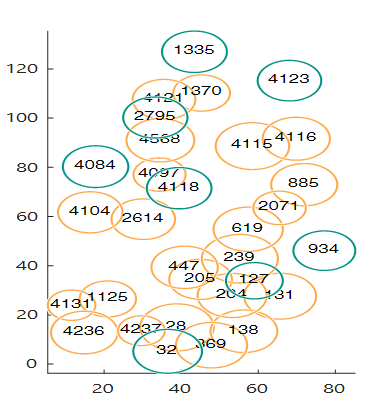
\includegraphics[width=\linewidth]{h1h2mosaic}
	\end{wrapfigure}
	A single data object to hold related Neurons. Inputs can be ID numbers or existing Neurons.
	\begin{lstlisting}[language=matlab]
	h1hc = sbfsem.NeuronGroup([28, 447, 619]);
	% Add a neuron to an existing group
	h1hc.add(4568);
	% Remove a neuron
	h1hc.remove(4568);\end{lstlisting} 
	The NeuronGroup class is still a work-in-progress. The current methods include:
	
	\paragraph{somaPlot} Plot the mosaic of somas
	\begin{lstlisting}[language=matlab]
	h1hc.somaPlot();
	h1hc.somaPlot('addLabel',true); % Label with ID
	h1hc.somaPlot('ax',gca); % Add to existing axis
	% Two methods for controlling plot color:
	h1hc.somaPlot('Color', [0 0.8 0.3]);
	h1hc.setPlotColor([0 0.8 0.3]); h1hc.somaPlot;\end{lstlisting}
	\paragraph{getSomaSizes} Return statistics on the soma sizes
	
	% -----------------------------------------------Subsection -- 
	\subsection{NeuronAnalysis}
	% -----------------------------------------------Subsection -- 
	The NeuronAnalysis class helps keep population data organized by managing input parameters and results of common analyses. To create a new analysis, subclass NeuronAnalysis and edit the \texttt{doAnalysis} and \texttt{visualize} methods.\\
	See \texttt{Tutorial.m} for information on these existing analysis classes:
	\begin{itemize}
		\item \textbf{DendriticFieldHull} - uses convex hull to estimate dendritic field area, includes methods for removing axons prior to analysis.
		\item \textbf{PrimaryDendriteDiameter} - returns the median dendrite diameter at a given distance from the soma.
	\end{itemize}
	% ------------------------------------------------- Section -- 
	\section{Views}
	% ------------------------------------------------- Section -- 
	Neurons can be passed to several UIs with the following syntax:
	\begin{lstlisting}[language=matlab]
	% VIEWNAME(NeuronObject);
	c6800 = Neuron(6800, 't');
	StratificationView(c6800);\end{lstlisting}
	\begin{itemize}
		\item \textbf{NodeView} - 3D scatter plot of cell and synapse annotations associated with a cell.
		\item \textbf{StratificationView} - Z-axis histogram of dendrites and synapses.
		\item \textbf{SomaDistanceView} - proxmial-distal distribution of dendrites and synapses.
	\end{itemize}
	\begin{figure}[h]
		\includegraphics[width=0.8\textwidth]{veiws}
	\end{figure}
	The checkboxes in the synapse table allow toggling the visibility of each synapse type. If the bin numbers in the synapse table are edited, the histogram plots will automatically update.
	% ------------------------------------------------- Section -- 
	\section{Images}
	% ------------------------------------------------- Section -- 
	% -------------------------------------------------- Figure -- 
	\begin{wrapfigure}{r}{0.3\linewidth}
		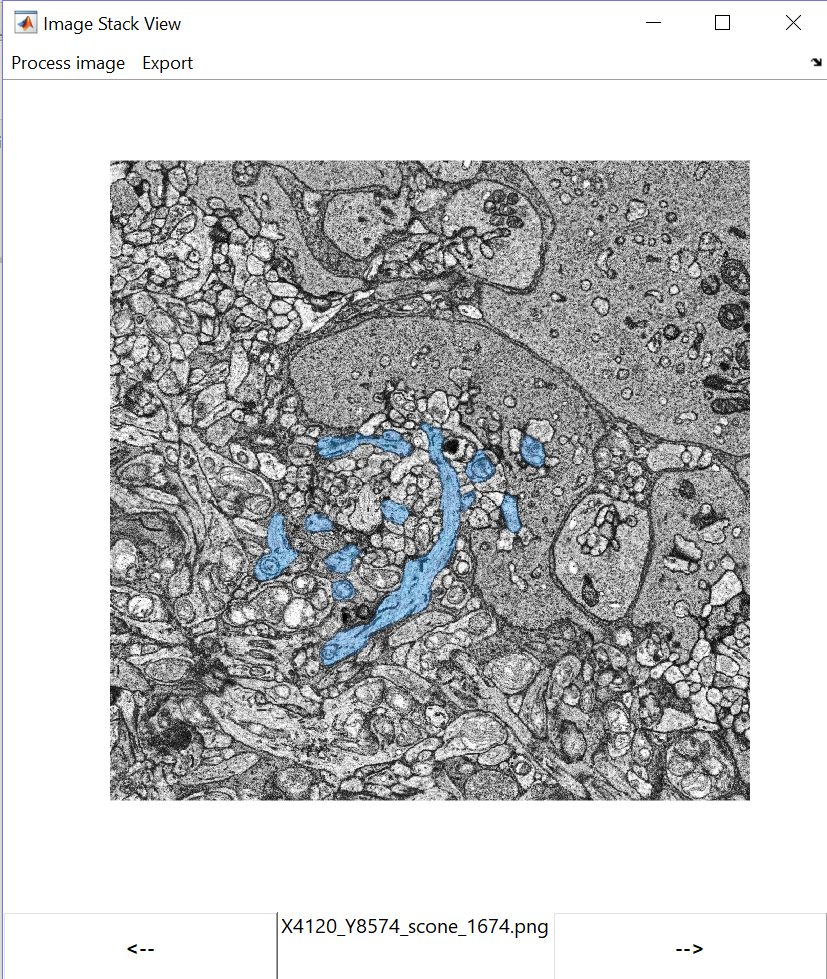
\includegraphics[width=\linewidth]{imstackapp}
	\end{wrapfigure}
	% -------------------------------------------------- Figure -- 
	% -----------------------------------------------Subsection -- 
	\subsection{ImageStackApp}
	% -----------------------------------------------Subsection -- 
	The ImageStackApp was built to scan through a series of images exported using Viking's Export Frames option (although this will work with any folder of images, provided there is some numbering in the file names). Pass a folder name to browse through the images (using left and right arrow keys or buttons). If the filenames contain numbers (Viking's export frames appends a frame number automatically), these will be used to order the images.
	\begin{lstlisting}[language=matlab]
	ImageStackApp('C:\...\foldername');\end{lstlisting}
	To crop the set of images, use \texttt{Process Image $\rightarrow$ Crop} and draw a rectangle on the image. Use \texttt{Full size} to return to the original size. Both changes require moving to another image to apply. 
	% -----------------------------------------------Subsection -- 
	\subsection{ImageStack class}
	% -----------------------------------------------Subsection -- 
	The ImageStackApp creates an ImageStack object. To create a GIF, create an instance of ImageStack alone and use the \texttt{stack2gif} function. 
	\begin{lstlisting}[language=matlab]
	I = sbfsem.images.ImageStack('C:\...\foldername');
	I.stack2gif();\end{lstlisting}
	% -----------------------------------------------Subsection -- 
	\subsection{Image Segmentation}
	% -----------------------------------------------Subsection -- 
	% --------------------------------------------Subsubsection -- 
	\subsubsection{Color ROIs}
	% --------------------------------------------Subsubsection -- 
	% -------------------------------------------------- Figure -- 
	\begin{wrapfigure}{r}{0.3\linewidth}
		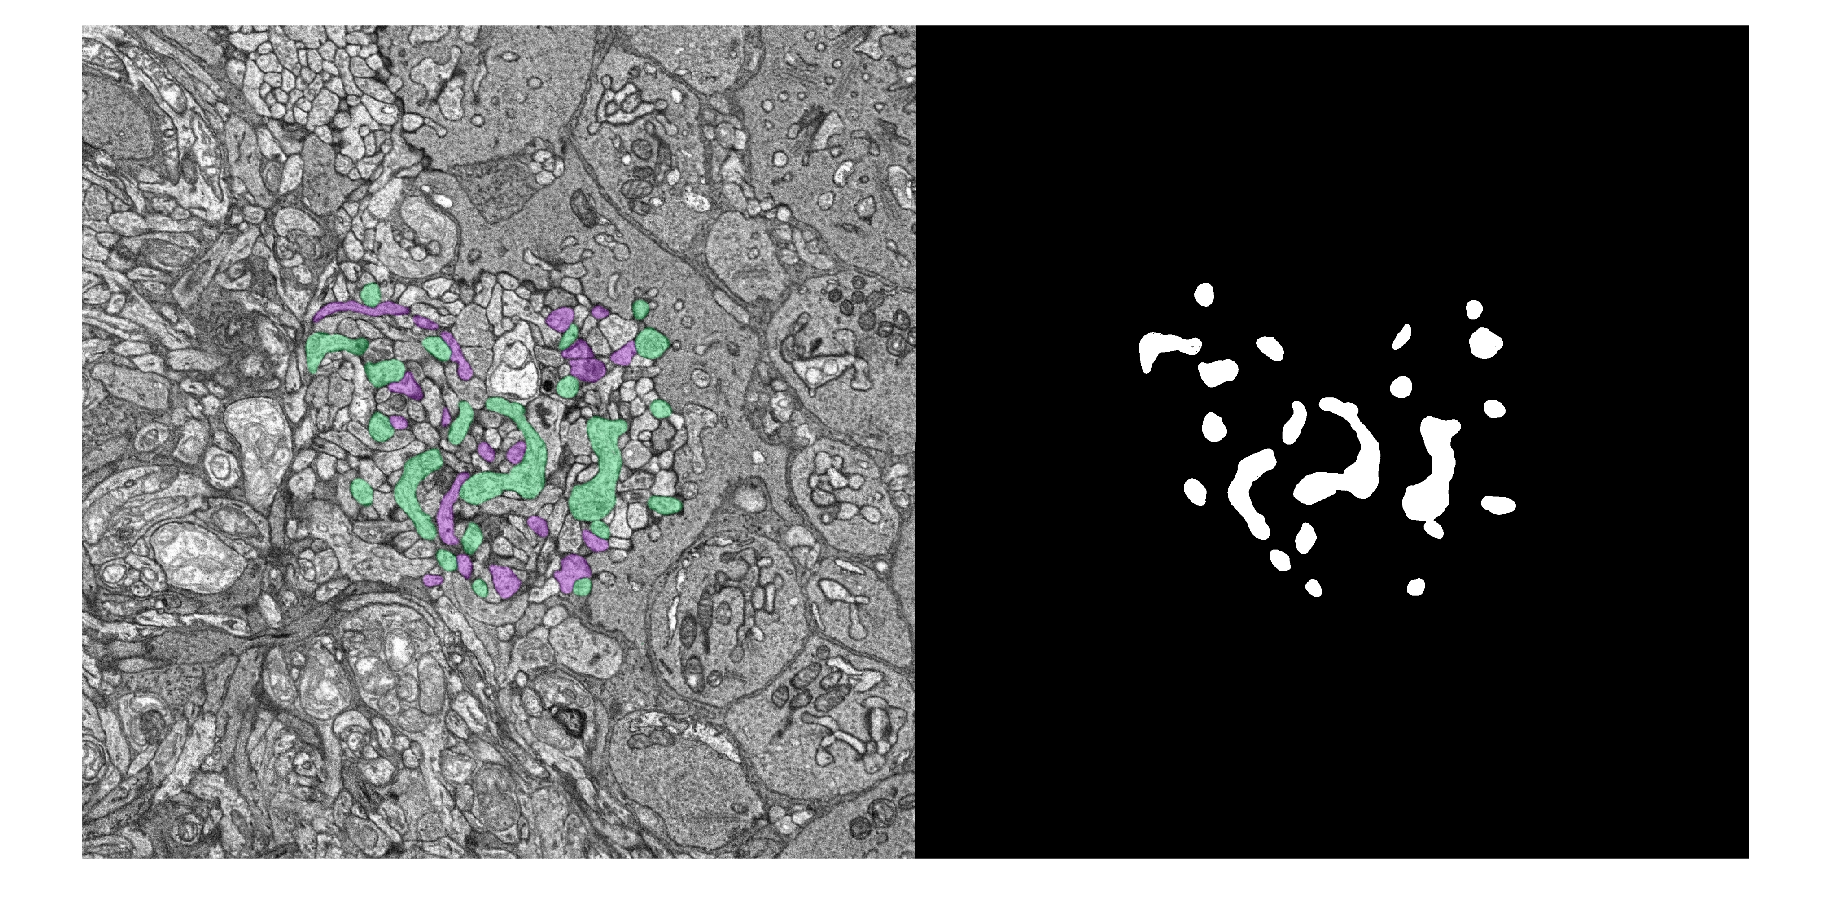
\includegraphics[width=\linewidth]{colorROI}
		\label{colorROI}
	\end{wrapfigure}
	% -------------------------------------------------- Figure -- 
	Renders can also be generated from a stack of EM images with color annotations. See \texttt{algorithms/segmentColorROI.m} for more information. Eventually I will make this more user-friendly. For now, new cell types and their thresholds must be added manually. To the right is an example of an L/M-cone with the ON- and OFF-midgets colored in Photoshop. On the right is the binary matrix output where 1/true (white) indicates a pixel within the color threshold limits.
	\subsubsection{Outlines}
	\texttt{getImageRGB.m} provides a quick tool for extracting data points from an image, given the outlines were drawn with a distinct color (red, green or blue in Paint works just fine). The first argument is the image, the second is the RGB value used to draw outlines.
	\begin{lstlisting}[language=matlab]
	pts = getImageRGB(im, [0 1 0]);
	\end{lstlisting}
	If more than one outline is present, MATLAB's \texttt{bwboundaries} can probably separate them into distinct objects.
	
	% ------------------------------------------------- Section -- 
	\section{Renders}
	% ------------------------------------------------- Section --
	% -----------------------------------------------Subsection -- 
	\subsection{Polygon Meshes}
	% -----------------------------------------------Subsection -- 
	% -------------------------------------------------- Figure -- 
	\begin{wrapfigure}{r}{0.25\linewidth}
		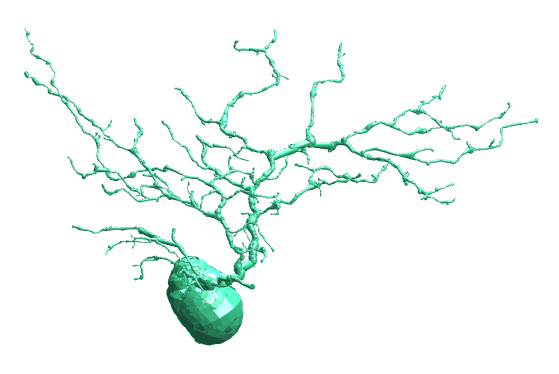
\includegraphics[width=\linewidth]{c6_render}
		\label{c6render}
	\end{wrapfigure}
	% -------------------------------------------------- Figure -- 
	Unlike the volumetric renders, the polygon meshes retain their absolute XYZ locations. This greatly simplifies the process of rendering multiple neurons to a single scene.
	\begin{lstlisting}[language=matlab]
	r1441 = sbfsem.render.Cylinder(Neuron(1441, 'i'));
	% If no axis handle is provided, creates new figure
	r1441.render();
	% Keep axis handle to direct next render to same figure
	ax = gca; 
	r1411 = sbfsem.render.Cylinder(Neuron(1411, 'i'));
	r1411.render('ax', ax, 'FaceColor', [0 0.8 0.3]);
	% Export as COLLADA .dae file
	r1411.dae();\end{lstlisting}

	A brief outline of the steps involved:
	\begin{enumerate}
		\item Query OData service for the all annotations in a given cell ID. Save the XYZ coordinates, radius and location ID of each annotation. 
		\item Query OData service for all links between annotations.
		\item Apply XY transforms to compensate for major shifts in section alignment.
		\item Query OData service for the volume dimensions - use these to convert XYZ coordinates and radius from pixels to microns.
		\item Convert the annotations and links between each annotation into the nodes and edges of an undirected graph.
		\item Create an undirected graph from all nodes (annotations/locations) and edges (location links).
		\item Use depth-first search (\texttt{dfsearch}) to divide nodes into segments of degree $=$ 2. This avoids rendering dendrite branches.
		\item Link each segment back to the parent node of degree > 2. This way some nodes are repeated but each edge is represented only once.
		\item Find the magnitude and angle of the distances between all connected nodes. Use this to get a quaternion rotation matrix for each edge.
		\item Input the radii to MATLAB's built-in 3D \texttt{cylinder} function, which creates a cylinder orthogonal to the XY plane.
		\item Rotate each node's cylinder by it's quaternion rotation matrix.
		\item Render each segment using surf - no lighting or edge color.
	\end{enumerate}
	% --------------------------------------------Subsubsection --
	\subsubsection{2D Projection}
	% --------------------------------------------Subsubsection -- 
	Rendering the above without any lighting creates a 3D figure with a 2D projection appearance.
	% --------------------------------------------Subsubsection --	
	\subsubsection{Blender Export}
	% --------------------------------------------Subsubsection --
	% -------------------------------------------------- Figure --
	\begin{wrapfigure}{r}{0.25\linewidth}
		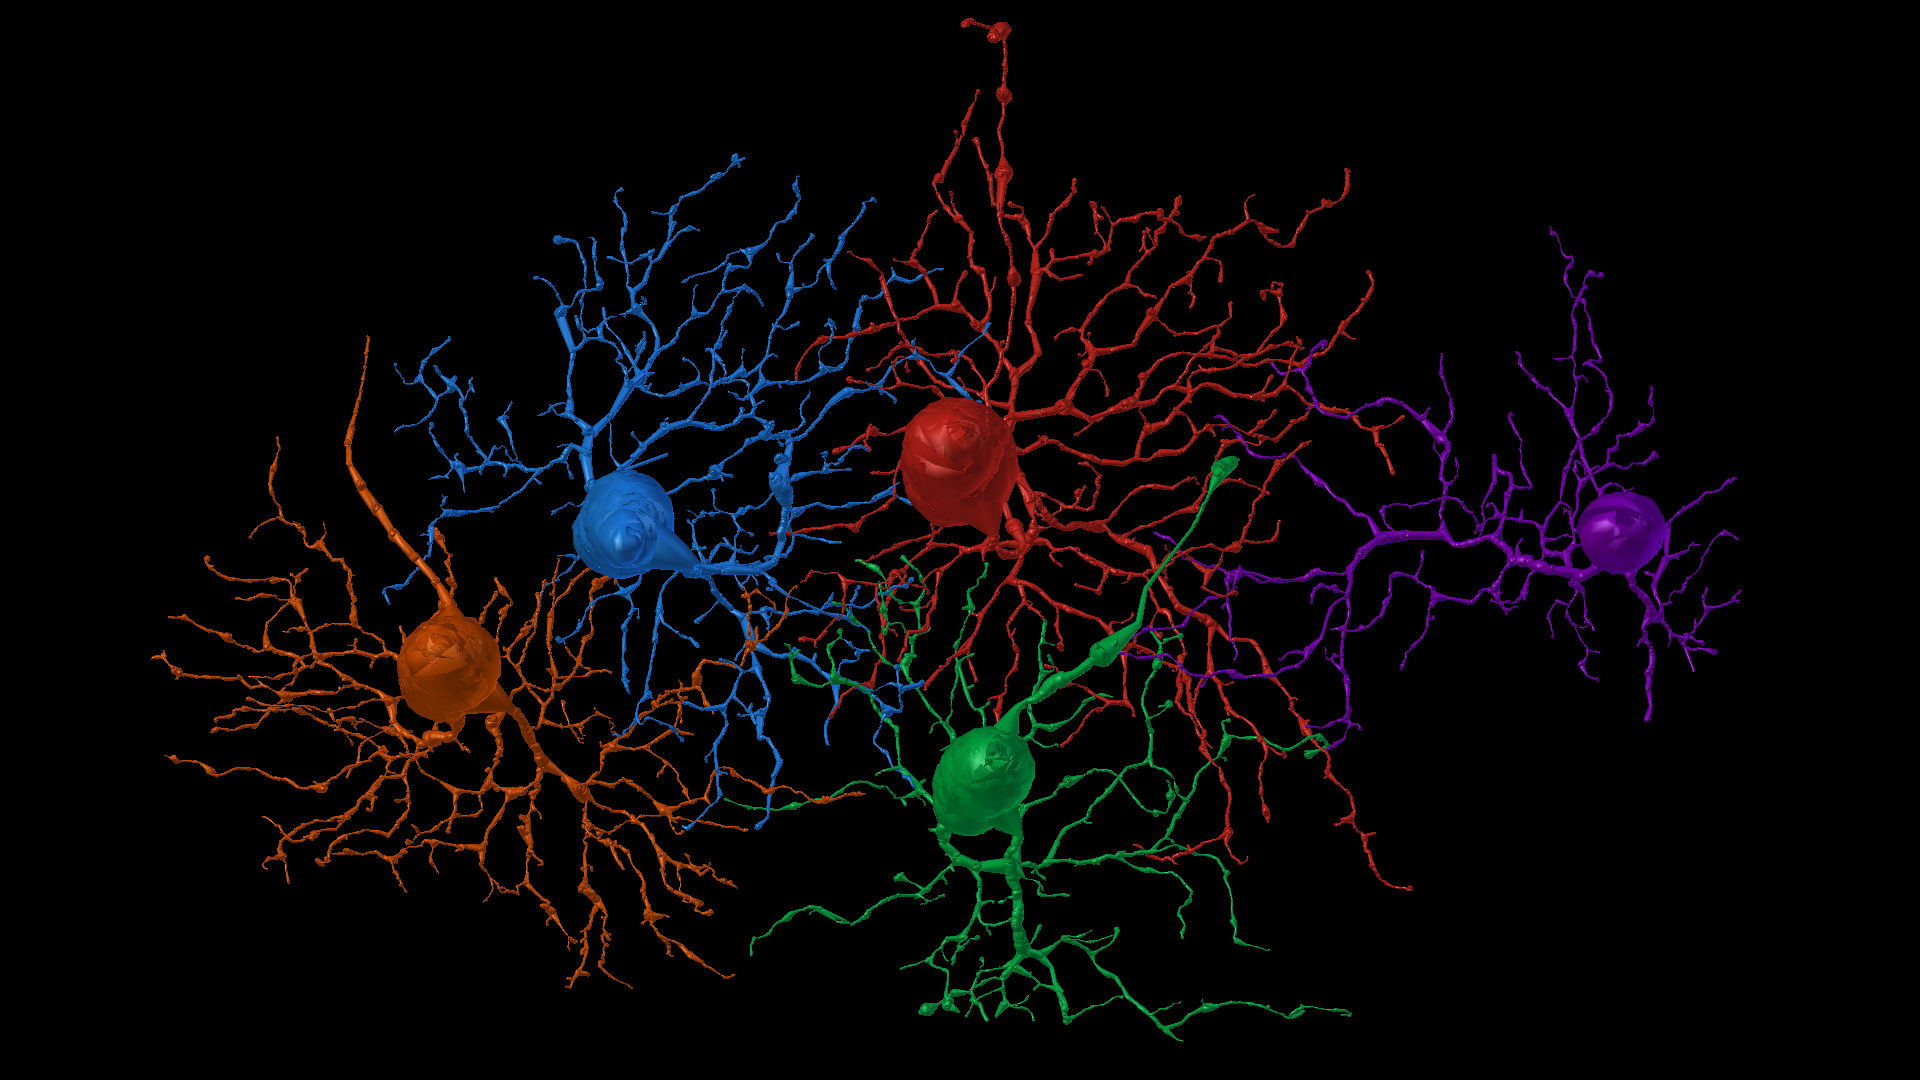
\includegraphics[width=\linewidth]{parasolRGCs}
		\label{blenderParasol}
	\end{wrapfigure}
	% -------------------------------------------------- Figure --
	To export the render to a COLLADA file, use:
	\begin{lstlisting}[language=matlab]
	r1411 = sbfsem.render.Cylinder(c1411);
	r1411.dae();\end{lstlisting}
	This function will open up a File Explorer window that allows you to select where to save the .dae file.\\

	In Blender, each .dae file must be imported separately through the \texttt{File $\rightarrow$ Import $\rightarrow$ Collada (default) .dae}. The relative positions of each neuron will be preserved as long as you import all the cells before rotating/transposing/scaling.\\
	The COLLADA export file is very minimal compared to VikingPlot. You will have to add a new Material for each cell (the \texttt{$+$ New} button in the Materials tab on the right panel). To optimize the final render, I then select \texttt{Smooth} for the Shading option in the Tools tab of the left panel. On the \texttt{Object Data} tab (directly to the left of the \texttt{Materials} tab), check both \texttt{Auto Smooth} and \texttt{Double Sided}. I move the \texttt{Angle} up to 50-60\si{degree} if the soma has especially sharp angles. Switching the view to Ortho (numpad 5) is helpful too.
	% -----------------------------------------------Subsection --
	\subsection{Volumetric Renders}
	% -----------------------------------------------Subsection --
	% --------------------------------------------Subsubsection -- 
	\subsubsection{Closed Curve}
	% --------------------------------------------Subsubsection --
	% -------------------------------------------------- Figure --
	\begin{wrapfigure}{r}{0.25\linewidth}
		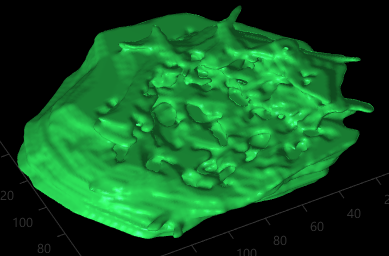
\includegraphics[width=\linewidth]{lmcone_render}
		\label{blenderParasol}
	\end{wrapfigure}
	% -------------------------------------------------- Figure -- 
	The closed curve renders support cutouts and multiple annotations per section. Mixing closed curve and disc renders is the next goal.
	\begin{lstlisting}[language=matlab]
	c2542 = Neuron(2542, 'i');
	lmcone = renderClosedCurve(c2542);
	% Decrease the resolution to speed up the renders
	lmcone = renderClosedCurve(c2542, 'resizeFactor', 0.5);\end{lstlisting}

	A basic outline of the code: 
	\begin{enumerate}
		\item Import control points for each Closed Curve annotation and parse into a 2xN matrix.
		\item Calculate a CatmullRom interpolating spline from the control points.
		\item Calculate a bounding box (the minimal volume containing all annotations)
		\item For each section, use \texttt{patch} to plot closed curves as white, cutouts as black and convert to a 2D binary matrix (similar to Figure \ref{colorROI}). 
		\item Resample
		\item Pad the 2D images as needed (occasionally the sizes will differ by 1 pixel) and stack into a 3D binary volume.
		\item Smooth the data (\texttt{smooth3} for now but there's much room for improvement here).
		\item Render using \texttt{isosurface} and \texttt{isonormals}.
		\item Set axis dimensions (\texttt{daspect}) according to volume dimensions pulled from OData service. 
	\end{enumerate}
	% --------------------------------------------Subsubsection -- 
	\subsubsection{Discs}
	% --------------------------------------------Subsubsection --
	% -------------------------------------------------- Figure -- 
	\begin{wrapfigure}{r}{0.075\linewidth}
		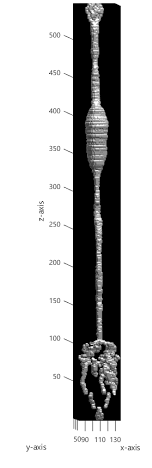
\includegraphics[width=\linewidth]{discBC}
		\label{discBC}
	\end{wrapfigure} 
	% -------------------------------------------------- Figure --
	The same method can be applied to Disc annotations as well for an accurate view of the annotations as discs in 3D. As is, the result is not as good as the polygon mesh rendering but could have some advantages in Blender.
	\begin{lstlisting}[language=matlab]
	c1893 = Neuron(1983, `i');
	r1893 = sbfsem.render.Disc(c1893);
	r1893.dae();\end{lstlisting}
	% -----------------------------------------------Subsection -- 
	\subsection{VikingPlot}
	% -----------------------------------------------Subsection -- 
	Editing the MATLAB figure generated by VikingPlot can be a good alternative to Blender. A few useful commands:
	\begin{lstlisting}[language=matlab]
	% Make sure the figure is the active window.
	ax = gca; % Create a handle to the axis
	ax.Children % Returns a list of child structures
	% There should be PATCH and LIGHT objects.
	% Use numerical indexing to generate handles to the objects
	% NOTE: The numbering might be different on your figure
	lightObj = ax.Children(1);
	renderObj = ax.Children(2);
	% A few useful properties to edit for PATCH objects:
	renderObj.FaceColor = [0, 0.8, 0.3];
	renderObj.FaceAlpha = 0.7;\end{lstlisting}
	% ------------------------------------------------- Section -- 
	\section{Image Registration}
	% ------------------------------------------------- Section --
	% -----------------------------------------------Subsection -- 
	\subsection{Section Misalignment}
	% -----------------------------------------------Subsection --
	\begin{wrapfigure}{r}{0.3\linewidth}
		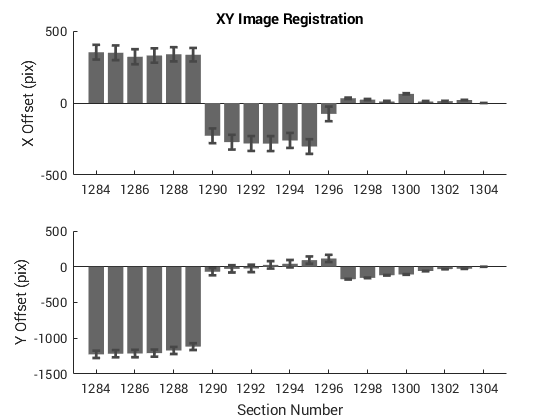
\includegraphics[width=\linewidth]{xyAlign}
	\end{wrapfigure}
	The function \texttt{xyRegistration.m} calculates the XY offset through a range of Z sections and outputs statistics on the offsets relative to the most sclerad section. The first output is an Nx3 matrix (columns = Section Number, XOffset, YOffset). A data file ($\mathtt{data/XY\_OFFSET\_NEITZINFERIORMONKEY.txt}$) tracks these offsets and can be updated using \texttt{updateRegistration.m}. The units are Viking's pixel coordinates. The transform is applied when the Neuron class first pulls X,Y coordinates from the OData service. 
	\begin{lstlisting}[language=matlab]
	[data, S] = xyRegistration('i', [1284 1309], true);
	updateRegistration('i', data);\end{lstlisting}
	This code is very new and needs quite a few improvements. However, the preliminary results are making a large difference in renders. See the code comments for more info.
	% -----------------------------------------------Subsection --
	\subsection{IPL Boundary Markers}
	% -----------------------------------------------Subsection --
	\begin{wrapfigure}{r}{0.25\linewidth}
		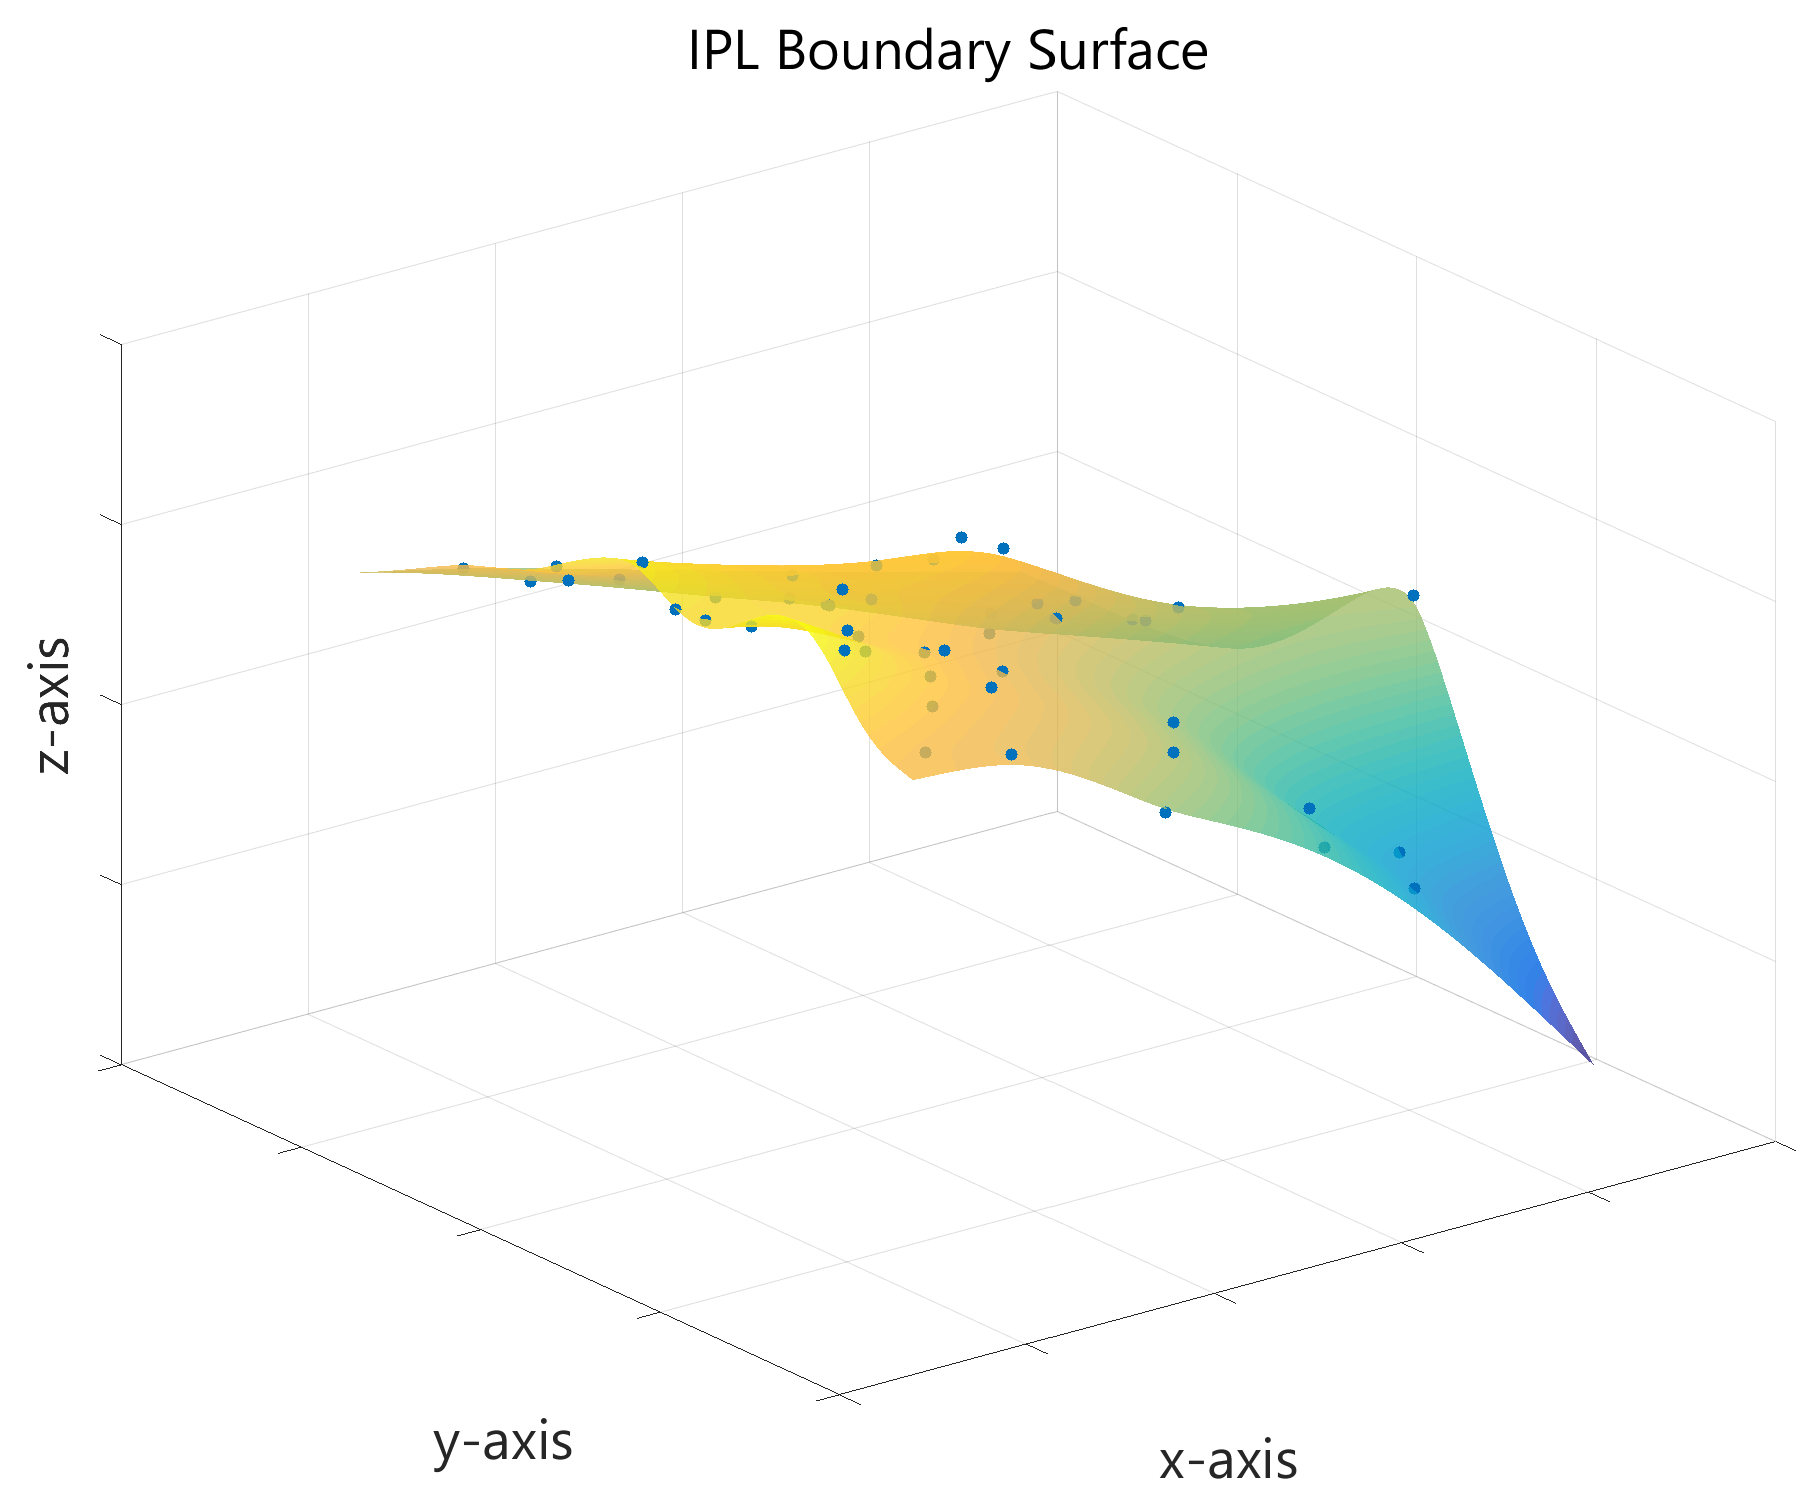
\includegraphics[width=\linewidth]{iplboundary}
		\label{iplboundary}
	\end{wrapfigure} 
	The INLBoundary and GCLBoundary objects retrieve all boundary markers in a given volume and create a surface to represent the slope of the tissue.
	\begin{lstlisting}[language=matlab]
	inl = INLBoundary('i');
	% Update marker locations from OData
	inl.refresh();
	% Create the surface
	inl.doAnalysis();
	% Plot the surface
	plot(inl);\end{lstlisting}
	Warping the Z-axis to account for the gradually sloping tissue is a goal. See IPL Boundary functions for generation of a surface based on depth markers. Soon I hope to have code to apply the transform - right now I'm thinking of adapting a commonly used method for warping neurons based on CHaT bands (\href{https://github.com/uygarsumbul/rgc}{Github repository}) \cite{Sumbul2014}.
	% ------------------------------------------------- Section -- 
	\section{Appendix}
	% ------------------------------------------------- Section --
	% -----------------------------------------------Subsection --
	\subsection{Matlab 101}
	% -----------------------------------------------Subsection --
	MATLAB tips are currently scattered throughout the documentation.. consolidate them here.\\
	Data structures like table, struct.\\
	Methods are class-specific functions. A list of all methods can be obtained by \texttt{methods(className)} (so, for example, \texttt{methods(`Neuron')}).
	% -----------------------------------------------Subsection --
	\subsection{Git 101}
	% -----------------------------------------------Subsection -- 
	Git can be downloaded \href{https://git-scm.com/}{here}. Once downloaded, you can open the terminal by right clicking anywhere in the whitespace of a File Explorer window and selecting \texttt{Git Bash here}. Do this in the folder you want sbfsem-tools to live in. 
	\begin{lstlisting}
	git clone http://github.com/sarastokes/sbfsem-tools.git\end{lstlisting}
	There should be a folder now called ``sbfsem-tools''. At any point, you can update the code to the latest version by right clicking on the folder itself, selecting \texttt{Git bash here} and typing in:
	\begin{lstlisting}
	git pull\end{lstlisting}
	This saves the step of deleting the existing sbfsem-tools folder and re-downloading it every time an update is available.
	% ------------------------------------------------- Section --	
	\begin{thebibliography}{[20]}
		\bibitem{Sumbul2014}
		Sumbul, U., Song, S., McCulloch, K., Becker, M., Lin, B., Sanes, J.R., Masland, R.H. \& Seung, H. S. (2014) A genetic and computation approach to structurally classify neuronal types. \textit{Nature Communications}, 5, 3512\\
		Github repository: \url{https://github.com/uygarsumbul/rgc}
	\end{thebibliography}
\end{document}